\documentclass[12pt]{report}

\usepackage[utf8]{inputenc}
\usepackage[T1]{fontenc}
\usepackage[francais]{babel}
\usepackage{multirow}
\usepackage{array}
\usepackage{color}
\usepackage{stmaryrd}
\usepackage{fancyhdr}
\usepackage{afterpage}
\usepackage{fullpage}
\usepackage{geometry}
\usepackage{setspace}
\usepackage{enumitem}
\usepackage[hyphens]{url}
\usepackage{hyperref}
\usepackage{wrapfig}
\usepackage{float}
\usepackage{graphicx}
\usepackage{tikz}
\usepackage{varwidth}


% Enlève les contours des liens
\hypersetup{
    linkbordercolor={1 1 1},
    citebordercolor={1 1 1},
    urlbordercolor={1 1 1},
    colorlinks=true,
    linkcolor=black,
    urlcolor=blue
}

% Custom colors
\definecolor{green-custom}{HTML}{70ad47}
\definecolor{blue-custom}{HTML}{5b9bd5}

% Redéfinis les marges des tableaux
\let\oldtabular=\tabular
\def\tabular{\small\oldtabular}
\renewcommand{\arraystretch}{1.5}


\title{\textbf{TA72 : Simulation d'atomes}}
\author{
    Aymen DAHECH \\
        \href{mailto:aymen.dahech@utbm.fr}{aymen.dahech@utbm.fr} \and
    Anthony RUHIER \\
        \href{mailto:anthony.ruhier@utbm.fr}{anthony.ruhier@utbm.fr}
}
\date{13 janvier 2017}

\pagestyle{fancy}
\setlength{\headheight}{12pt}
\fancyhf{}
\fancyhead[L]{Aymen DAHECH, Anthony RUHIER}
\fancyhead[R]{Simulation d'atomes}
\geometry{headsep=5ex}

\graphicspath{{graphics/}}
\usetikzlibrary{arrows,positioning}

\setlength{\intextsep}{0pt}

\begin{document}

{
\newgeometry{left=1cm,right=1cm,bottom=3cm,top=1cm}
\begin{titlepage}

\vbox to 70pt{\hfill
\includegraphics[height=2cm]{logo-utbm.eps}}\
\begin{center}

\textsc{\LARGE Université de technologie Belfort-Montbéliard}\\[0.7cm]
\textsc{\LARGE Département Informatique}\\[1.0cm]
\textsc{\Large TA72 -- Projet Tutoré}\\[5cm]


% Title
{ \huge \bfseries Conception d'une simulation d'atomes}\\[0.5cm]
{ \huge \bfseries Rapport général}\\[3cm]

% Author and supervisor
\begin{large}
Aymen \textsc{Dahech} \\
    \href{mailto:aymen.dahech@utbm.fr}{aymen.dahech@utbm.fr}\\[1em]
Anthony \textsc{Ruhier} \\
    \href{mailto:anthony.ruhier@utbm.fr}{anthony.ruhier@utbm.fr}\\[1em]

\end{large}

\vfill

% Bottom of the page
{\large 13 janvier 2017}

\end{center}
\end{titlepage}
}

% Hack to force a new page
{\clearpage\mbox{}\thispagestyle{empty}\clearpage}
\setcounter{page}{1}

\thispagestyle{empty}
\vspace{4em}
\tableofcontents

\afterpage{\cfoot{\thepage}}
\newpage

%%%% Includes des chapitres :
%%%%%%%%%%%%%%%%%%%%%%%%%%%%%%
\setcounter{page}{1}
\chapter*{Introduction}

\addcontentsline{toc}{chapter}{Introduction}

\paragraph{}
Dans le milieu pétrochimique ou dans la chimie pédagogique, nous assistons à
une réelle demande d'outils de simulations d'éléments à vue moléculaire ou
atomique: une représentation graphique d'une réaction permet une meilleure
compréhension de celle-ci, et facilite l'apprentissage en complétant les
maquettes, souvent utilisées.

\paragraph{}
Pour répondre à ce besoin, dans le cadre de notre projet tutoré dans l'Unité de
Valeur TA72, nous avons entamé la conception d'un outil de simulations
graphique d'atomes sous la tutelle de Monsieur Fougères. Nous ne nous
démarrions pas le projet de zéro puisqu'il a également fait l'objet du projet
de fin de semestre de l'UV LP74, suite à laquelle nous nous sommes vus proposer
de le continuer.

\paragraph{}
Tel que laissé en LP74, l'outil affichait une représentation 3D d'un
environnement d'atomes, se déplaçant de manière aléatoire mais gérant les
collisions. L'utilisateur pouvait se déplacer dans l'environnement pour
visualiser les atomes. Quelques problèmes de performances étaient présents,
certains provoquant des crashs de l'application.

\chapter{Présentation du sujet}
\label{presentation_sujet}

\section{Objectifs}

\paragraph{}
Le but du projet a été de continuer le travail entrepris via la première
version de l'application afin d'obtenir trois niveaux de vues (atome, molécule
et réaction), un design en agents et des mouvements d'atomes plus réalistes qui
sont soumis à des lois d'attraction/répulsion


\section{Aperçus}

\paragraph{}
Voici différents aperçus de l'application réalisée :

\begin{figure}[H]
\centering
\centerline{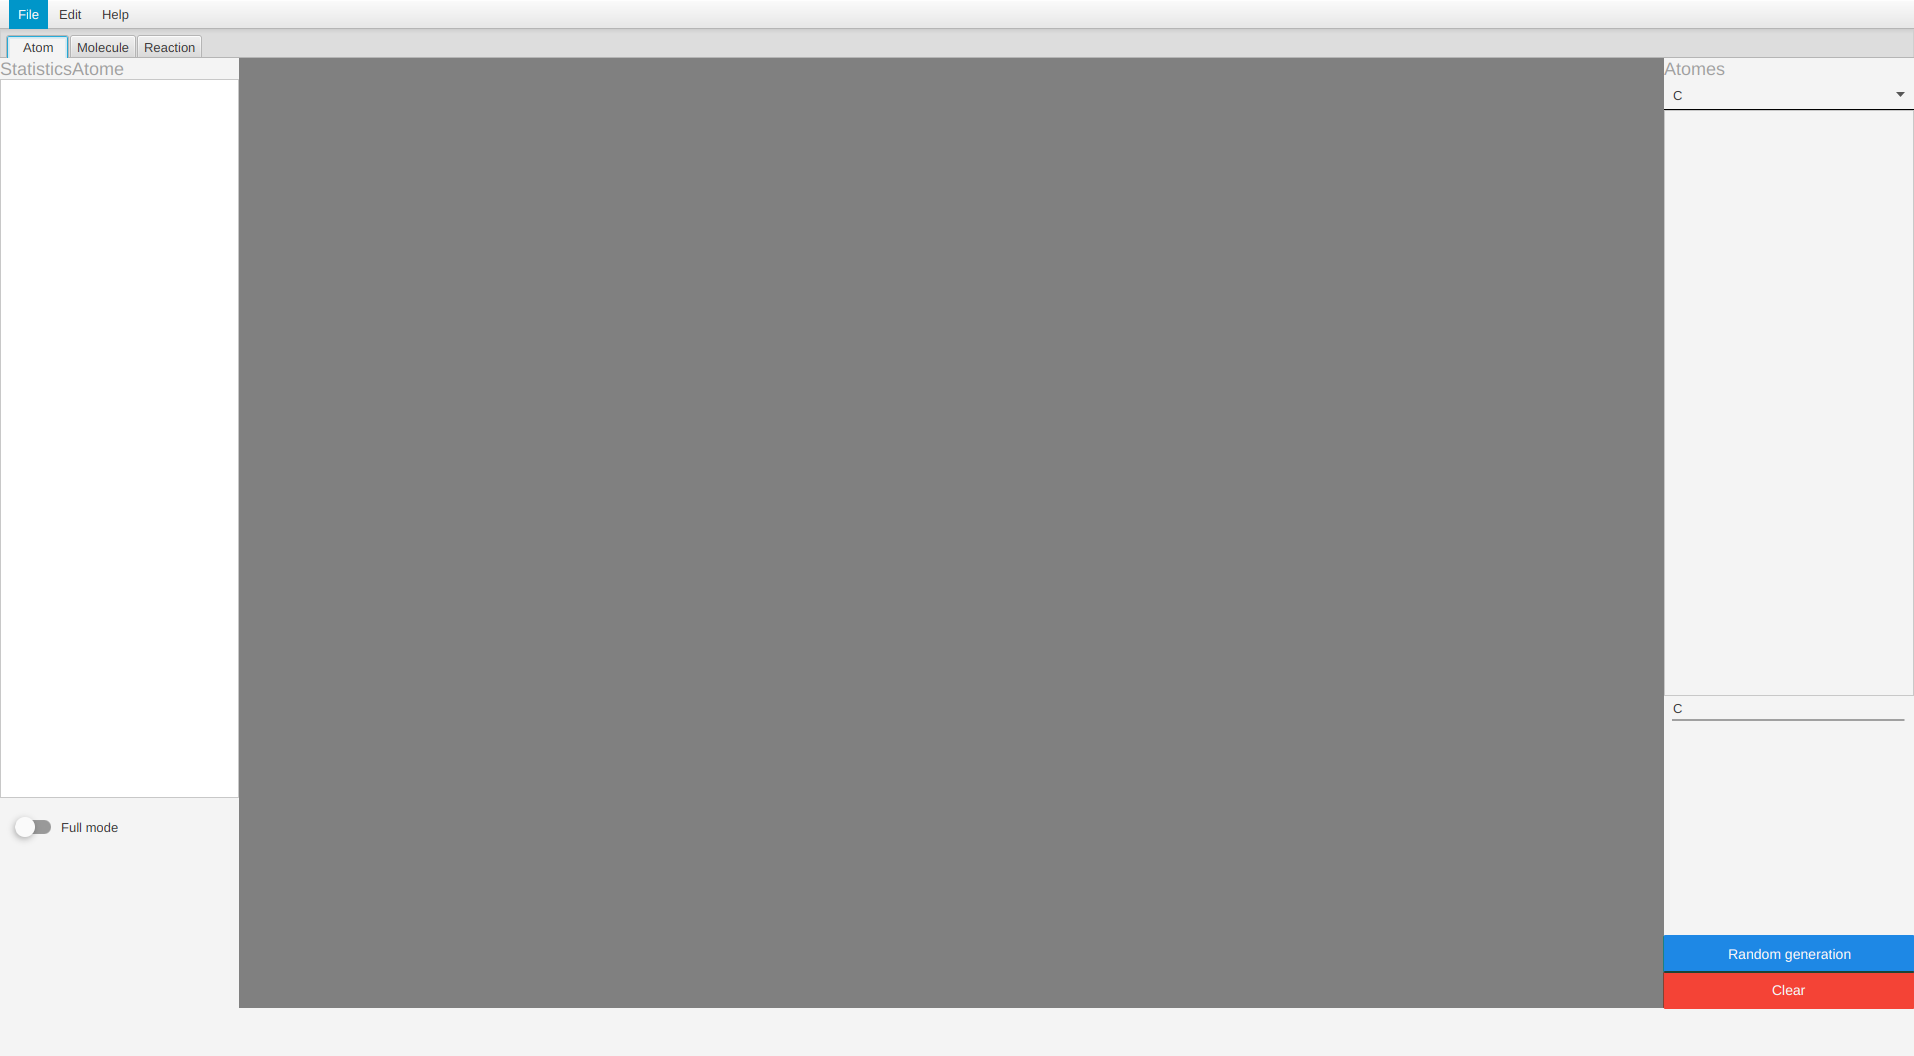
\includegraphics[width=1.2\textwidth]{screenshot_atom}}
\caption{Vue sur l'onglet Atome}
\label{screenshot_atom}
\end{figure}

\paragraph{}
La vue Atome permet normalement de générer un atome et de le visualiser.
Cependant, à la fin de cette TX, il n'est pas encore fonctionnel.

\begin{figure}[H]
\centering
\centerline{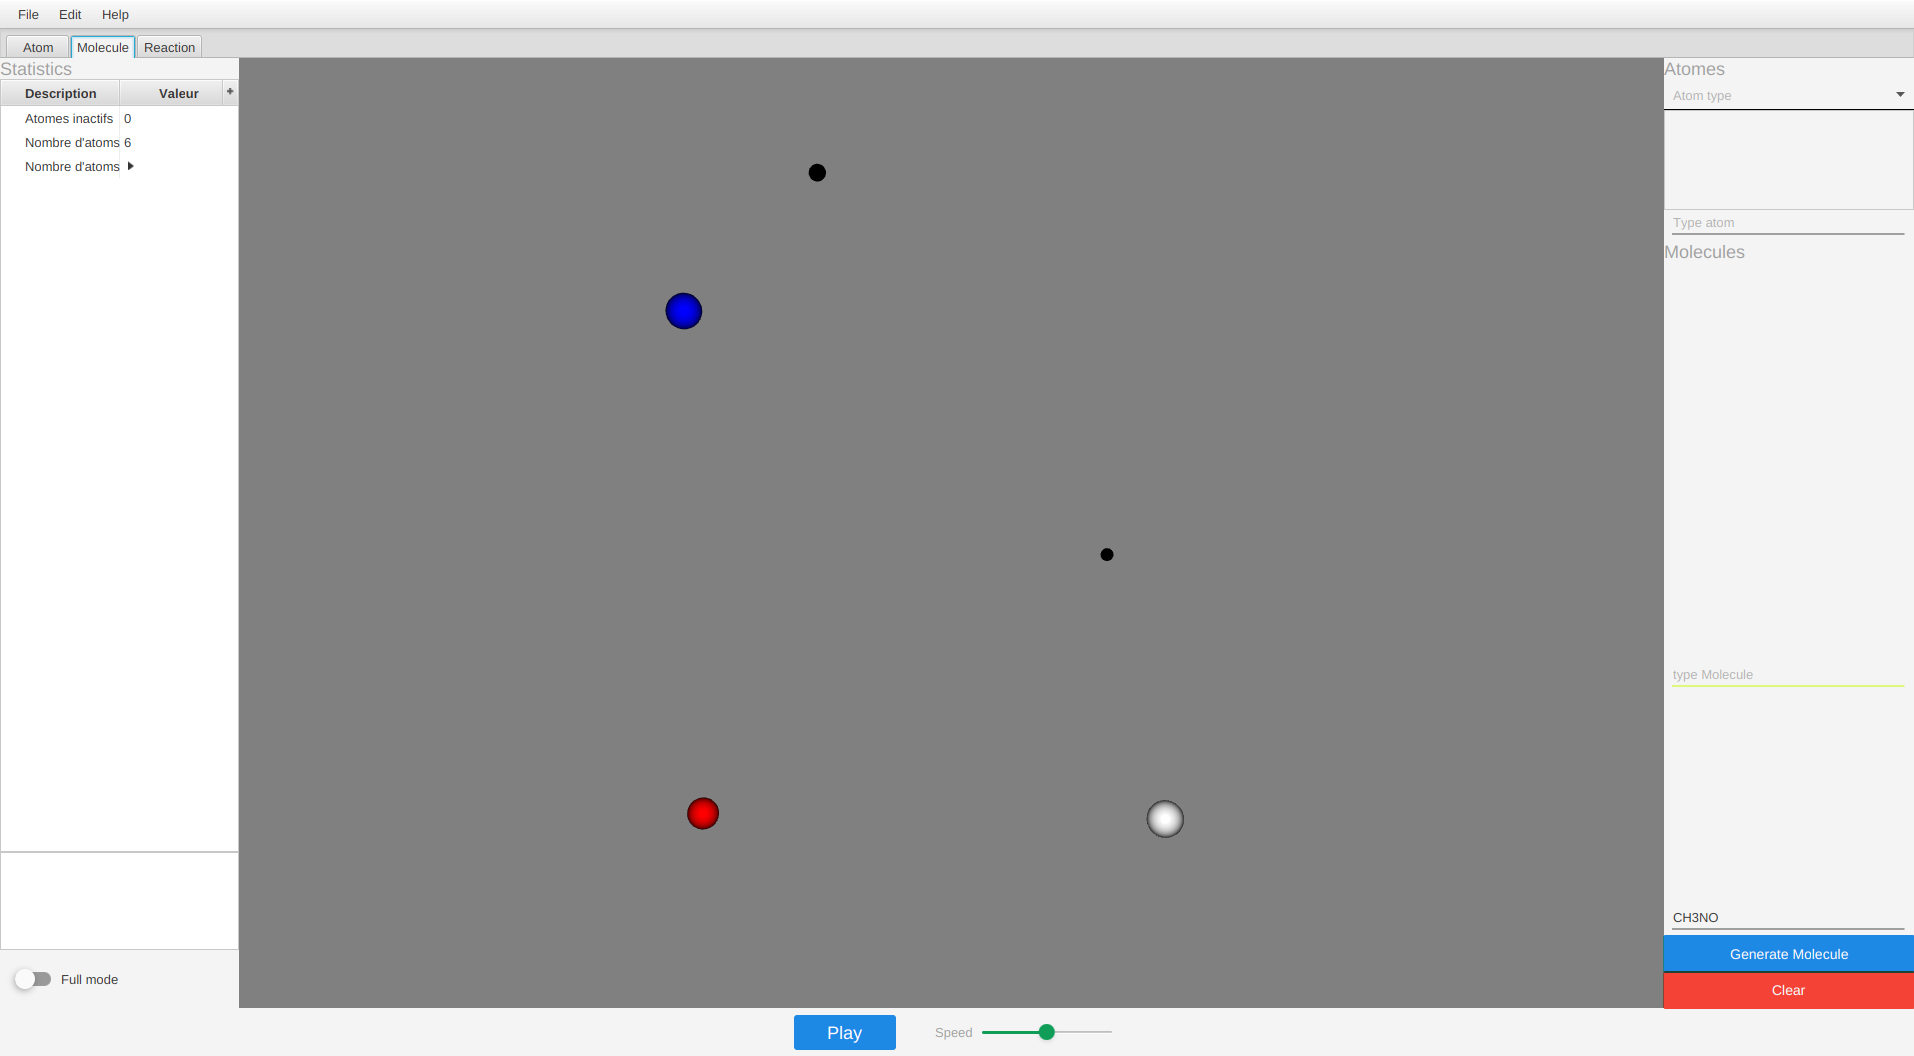
\includegraphics[width=1.2\textwidth]{screenshot_molecule}}
\caption{Vue sur l'onglet Molécule}
\label{screenshot_molecule}
\end{figure}

\paragraph{}
La vue Molécule permet de générer une molécule depuis une formule et de la
visualiser.


\begin{figure}[H]
\centering
\centerline{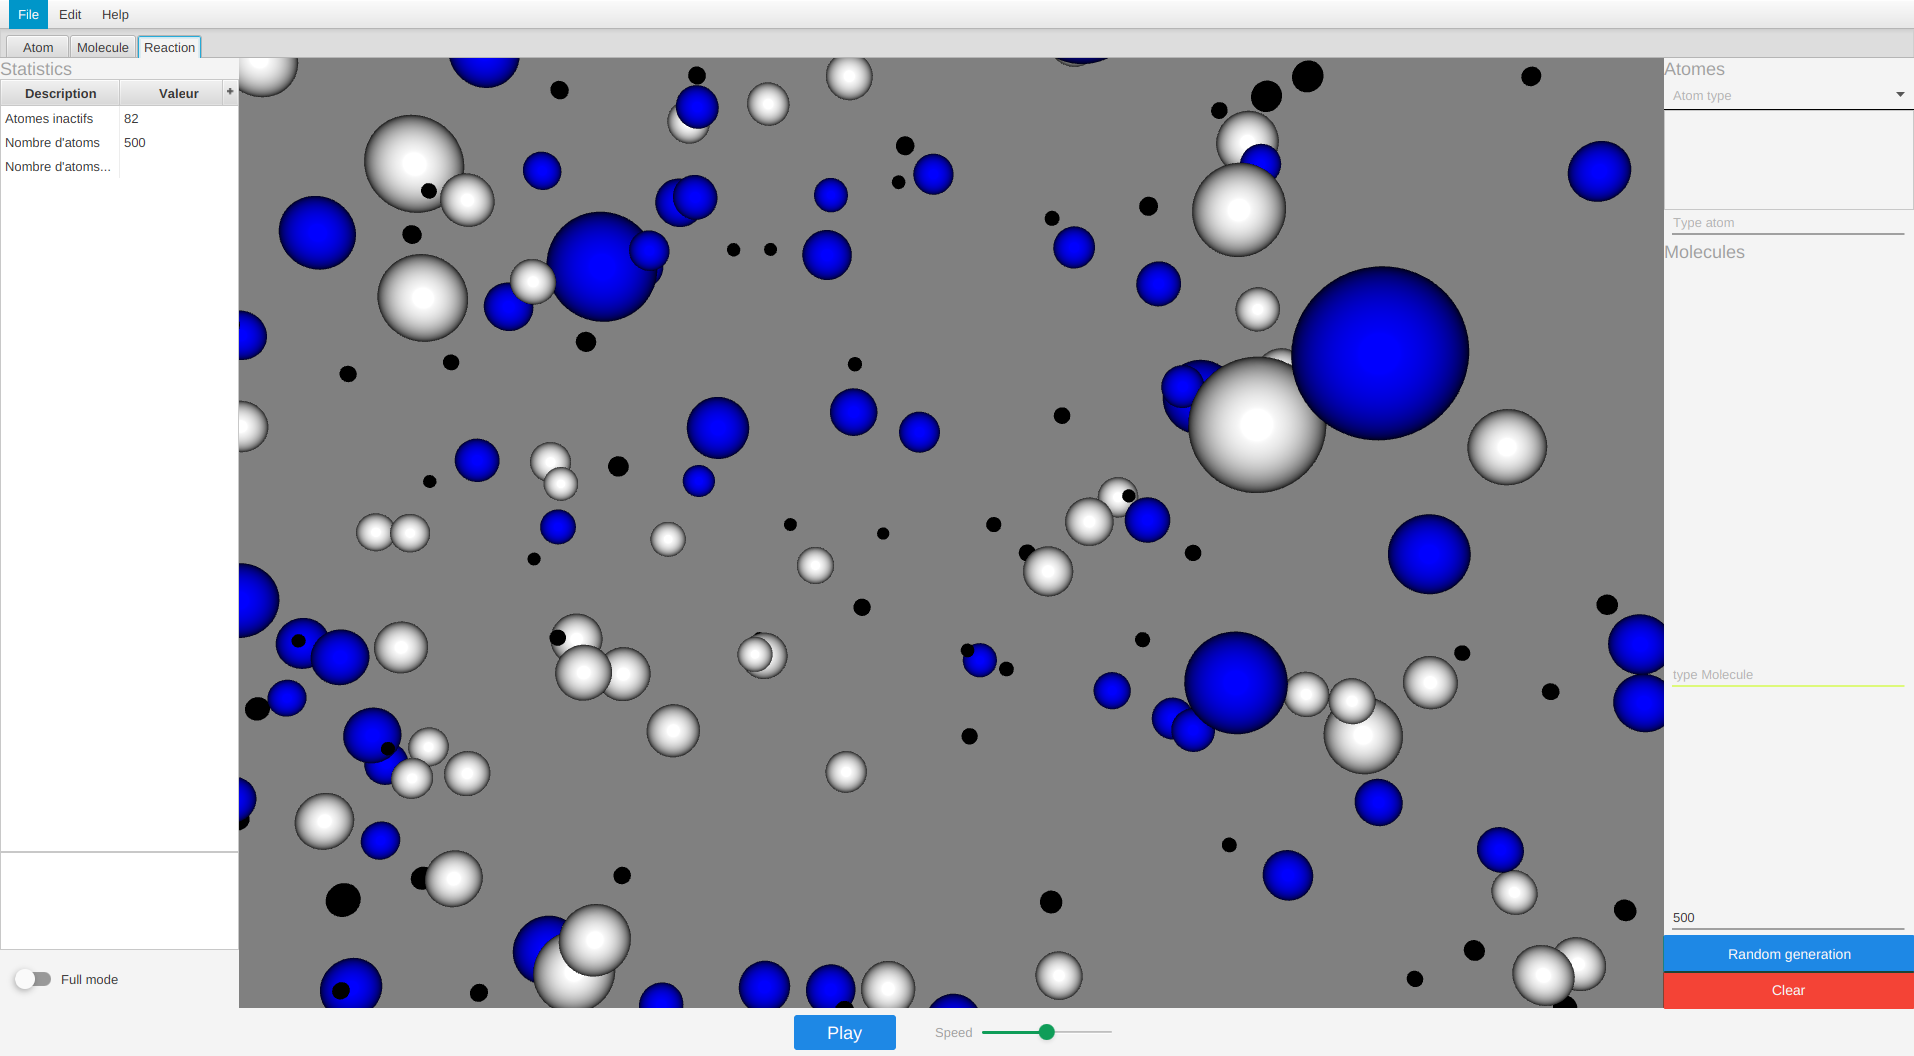
\includegraphics[width=1.2\textwidth]{screenshot_reaction}}
\caption{Vue sur l'onglet Réaction}
\label{screenshot_reaction}
\end{figure}

\paragraph{}
La vue réaction permet de générer un ensemble d'atomes, réagissant ensemble en
formant des molécules via un système d'attraction/répulsion.

\chapter{Mise en oeuvre}
\label{mise_en_oeuvre}

\section{Analyse de l'existant}

\paragraph{}
Dans une optique d'amélioration de l'existant, un bilan sur l'application telle
que rendue en LP74 a été effectué.


\subsection{Application dans un unique thread}

\paragraph{}
Le dessin des atomes, la gestion de leurs déplacements mais ainsi que toute
navigation dans l'interface sont effectués dans un unique thread.

\paragraph{}
Les atomes et molécules sont stockées dans une liste chainée, parcourue de
manière continue et séquentielle par l'application pour mettre à jour leurs
coordonnées. Il est alors nécessaire que le calcul des nouvelles coordonnées
ainsi que le dessin de chaque sphère soient simples et rapides pour rester
inférieur à la durée d'une frame, afin obtenir des mouvements fluides.

\paragraph{}
De cette manière, les atomes n'étaient pas indépendants : un objet
Environnement coordonne l'ensemble, et force de lui-même les mises à jour des
informations.  Il a également comme rôle de vérifier les collisions.


\subsection{Consommation excessive de mémoire}

\paragraph{}
L'application souffre de problèmes de consommation mémoire, avec des fuites
dues à JavaFX (le framework graphique utilisé) qui amènent des lenteurs.
L'application se fige par moments, et il arrive également qu'elle se fasse
tuer par l'OOM killer du système.


\subsection{Mouvement strictement basés sur de l'aléatoire}

\paragraph{}
Les mouvements des atomes ne sont pas basés sur des attractions ou répulsions
entre éléments. L'application impose un aspect ``brouillon'' dans les vecteurs
vitesses des éléments, de façon à donner l'impression que l'environnement n'est
pas uniforme. Tout repose sur un système aléatoire, avec gestion de collisions
et inversions de vecteurs vitesses lorsqu'un élément s'approche de trop près
des bords du bac.


\subsection{Formations de molécules}

\paragraph{}
De façon à former des molécules, et contrairement à ce qui est indiqué dans la
partie liée aux mouvements, une sorte d'attraction a été mise en place. Nous ne
considérons pas que le système en place soit suffisamment exact pour qu'il ait
une réelle influence sur les mouvements des atomes.

\paragraph{}
Néanmoins, si la vitesse d'un atome est suffisamment faible et qu'il rentre en
collision avec un autre atome, ces deux atomes vont se lier. La liaison ne
repose sur rien de scientifique, dans le sens où, par exemple, les couches de
valences ne sont pas prises en compte. Aucune vérification n'est effectuée
pour savoir si les atomes peuvent réellement se lier entre eux.

\chapter*{Conclusion}

\addcontentsline{toc}{chapter}{Conclusion}

\paragraph{}


\end{document}
